\documentclass{article}
\usepackage{multirow}
\usepackage{hyperref}
\usepackage{graphicx}
\usepackage{xcolor}
\usepackage{float}
\usepackage{setspace}
\usepackage[a4paper]{geometry}
\usepackage[numbers,sort]{natbib}

\title{Root Digger: a root placement program for phylogenetic trees}
\author{Ben Bettisworth, Alexandros Stamatakis}
\date{\today}

\newcommand{\RootDigger}{RootDigger}
\newcommand{\RootDiggertt}{\texttt{RootDigger}}
\newcommand{\BenComment}[1]{{\bf \color{blue} ({#1})}}
\newcommand{\AlexisComment}[1]{{\bf \color{green} ({#1})}}
\doublespace

\begin{document}
\begin{abstract}
  In phylogenetic analysis, it is common to infer trees which are unrooted.
  This is to say, it is unknown which node is the most recent common ancestor of
  all the taxa present in the phylogenetic tree.
  This information is often desirable, as it provides a direction to the edges in
  the tree.
  There exist several methods to recover a root, including midpoint rooting and
  using a special taxon as a so called outgroup.
  Additionally, a non-reversable Markov model can be used to compute the
  likelihood of a root.
  In this paper, we present software which uses a provided non-reversable model
  to compute the most likely root location.
\end{abstract}

\maketitle

% Main Points:
% - Rerunning analysis with outgroups is expensive, and can introduce errors
% - Midpoint rooting is a joke
% - This is fast and accurate.

\section{Introduction}

% Outline:
% - What is rooting
% - Why do we need it
% - Existing methods
% - What this method is
% - Why should we use this method

When inferring phylogenetic trees, most phyogenetic inference tools
\cite{nguyen_iq-tree:_2015, stamatakis_raxml_2014, minh_iq-tree_2019} will infer
an unrooted tree. This is due to a standard for phylogenetic tools assumption:
reversibility of the character substitution process
\cite{felsenstein_evolutionary_1981}.  This yields the problem of inferring a
phylogenetic tree computationally tractable.  However, by making this assumption
the ability to identify a root is lost. A rooted phylogenetic tree is desirable,
though, as it can resolve long standing disputes regarding the placement of
large clades on the tree of life \cite{dunn_animal_2014} for example.

There are several methods to recover the root on an existing phylogenetic tree,
which generally fall into one of three categories: methods which use additional
topological information not present in the molecular data; methods which
utilize some variation of the molecular clock hypothesis; and methods which use
a non-reversible model.
\doublespace

Methods that use additional topological information take advantage of prior
knowledge about the world, which is not present in the data that is used to
infer the tree. In particular, knowledge about species which are distantly
related can be used to add a so-called outgroup to phylogenetic analysis.  This
outgroup can then be used to place the root on the tree, as the most recent
common ancestor of the ingroup and the outgroup must be the root of the tree.

There are challenges to adding an outgroup to an analysis.  Gatsey et. al.
\cite{gatesy_how_2007} showed how adding a single taxon to an analysis can
substantially change the resulting tree topology, even for the taxa which were
already present in the analysis before (i.e., the ingroup).  Holland
\cite{holland_outgroup_2003} investigates this phenomenon in simulations, and
finds that outgroups that affect or alter the topology of ingroups are common.

Alternatively, molecular clock analysis can be used to place a root without
prior topological knowledge \cite{yang_computational_2006}.  The molecular clock
hypothesis states that base substitution ``ticks'' at a stochastically constant
rate.  Using this assumption, or some variant thereof, a likely location can be
inferred for the root on an existing phylogenetic tree.  A simple version of
this is midpoint rooting, which uses a constant molecular clock assumption.

Molecular clock analyses exhibit their own difficulties. In particular, the
clock does not "tick" at a constant rate over the tree as shown in
\cite{li_molecular_1987} and \cite{steiper_primate_2006}. Relaxed clock models
exist which can alleviate this problem, but are not always successful at
correctly identifying the root as shown in \cite{battistuzzi_performance_2010}.

The final method that can place a root on a tree is to perform the phylogenetic
analysis using a non-reversible model. By using a non-reversible model, we can
place a direction of time on the branches of a tree \cite{yap_rooting_2005}.
Several software packages are able to infer a phylogenetic tree under a
non-reversible model, and thereby inferring a root \cite{nguyen_iq-tree:_2015,
ronquist_mrbayes_2003}.

Non-reversible models for phylogenetic trees come in many forms.  For example,
accounting for duplication, transfer, and loss events yields a non-reversible
model \cite{morel_generax:_2019}.  In particular, duplication events have been
used for rooting trees \cite{emms_stride:_2017}.  Another method, the one primarily
used in this work, is to eliminate the reversibility assumption of standard
character (e.g., nucleotide or amino acid) substitution models.  Unfortunately,
eliminating this assumption significantly increases the computational effort
required to find a good (high likelihood) phylogenetic tree.  This is due to the
loss of the pulley principle \cite{felsenstein_evolutionary_1981}, which allows
phylogenetic inference tools to ignore placement of the root during tree
inference.  Therefore, by adopting a non-reversible model, the location of a
root on a phylogenetic tree affects the likelihood of that tree.

Since the location of the root affects the likelihood of the tree, while using
standard tree search techniques all possible rootings would need to be evaluated
for each tree in order to find the rooting with the highest likelihood.  In the
worst case, this increases the work {\em per tree} by a factor of
$\mathcal{O}(n)$ where $n$ is the number of taxa present in the dataset.
Eliminating the reversibility assumption drastically increases the computational
effort required to infer a tree. Therefore, standard inference tools choose to
adopt the reversiblity assumption, as phylogentic tree inference would be
computationally intractable otherwise.

As an alternative to the computationally expensive process of inferring a tree
with a root, an unrooted tree which has already been inferred under a reversible
model can be evaluated a posteriori for possible root locations under a
non-reversible model.  This is less computational effort, as it skips the
expensive step of looking for ``good'' rootings in intermediate trees during the
tree search.  With this method, we can find the most likely root location for a
given phylogenetic tree.  Even with this method there are still numerical
challenges, as the likelihood function for rooting a phylogenetic tree may
exhibit several local maxima \cite{huelsenbeck_inferring_2002}, although we did
not find this to be a major concern in our experiments (see the discussion).

We implemented the open source software tool \RootDiggertt{} which uses a
non-reversible model of character substitution to infer a root on an already
inferred tree. The inputs to our tool is a multiple sequence alignment, and a
phylogenetic tree, and produces a rooted tree. \RootDiggertt{} implements fast
and a slow modes, called Search mode and Exhaustive mode, respectively. The
search mode simply finds the most likely root quickly. The exhaustive mode
evaluates the likelihood of the root for every branch of a given tree, and
reports the likelihood weight ratio \cite{strimmer_inferring_2002} for placing a
root on that branch for every branch on the tree. In addition to the two search
modes, there is an optional early stop mode, which can be combined with either
rooting mode. In this early stop mode, the search will conclude if the root
placement is nearly the same twice in a row. This is to say, if the location of
the best root position is on the same branch as the previous iteration {\em and}
the value inferred for the root position is sufficiently close, then the
objective function is considered satisfied, and the current iteration
terminates.  While the early stop optimization does improve rooting times
substantially (around 1.7 times faster), the likelihood of the root placement
will not be fully optimized.  In practice, this does not substantially effect
the final root placement, but it does render comparison of the likelihood with
results from other tools impossible.

\section{Methods}

The input to \RootDiggertt{} is a multiple sequence alignment (MSA) and a
phylogenetic tree with branch lengths in expected mean substitutions per site.
\RootDiggertt{} then uses the tree and branch lengths to find the most likely
root location by calculating the likelihood of a root location under a
non-reversible model of DNA substitution (specifically, UNREST
\cite{yang_estimating_1994}). The optimal position of the root along a branch is
calculated by splitting the given branch in two branches with resulting branch
lengths $\alpha t$ and $(1-\alpha) t$, $0 \leq \alpha \leq 1.0$.  We then find
the maximum likelihood value of $\alpha$, and report the likelihood for given
branch as the likelihood of the root location.  By formulating the problem this
way, we can use single parameter optimization techniques such as Brent's
Method\footnotemark{}, which are computationally more efficient compared to
multi-parameter optimization routines.

\footnotetext{
  Brent's Method is picked over Newton's Method because it does not require a
  second derivative to optimize the funciton.

  We computed an analytical version of the second derivative, but the library
  that we use doesn't support calculating some of the values involved.
  The effort to rewrite the functions that would compute these values
  deemed to be too much relative to the savings.
  In principle, the computation could be done.
}

A quirk of Brent's and similar methods is that they find extrema by finding
roots for the objective function's derivative. In order to find maxima, though,
it is required that the objective function's value is checked. In addition,
Brent's method will fail to find all extrema.  To compensate, we need to search
for bracketing windows that can be used to safely find extrema.  Unfortunately,
we are not aware of a general method for finding such bracketing windows, so a
recursive method is employed, were the search range is reduced in half and
searched for appropriate\footnotemark{} windows.

\footnotetext{Appropriate here means that the sign of the function in question
  has opposite signs at the endpoints of the window.}

As mentioned in the introduction, \RootDiggertt{} has 2 modes of operation.
These modes will be discussed individually, starting with placement mode:

\begin{enumerate}
  \item Initialize numerical model parameters:
        \begin{itemize}
          \item $\alpha$-shape parameter for rates to $1.0$ (if applicable),
          \item Character substitution rates to uniform random values according
                to $U(0.0001, 1.0)$,
          \item Base frequencies to uniform random values according to
                $U(0.0001, 1.0)$, which are then normalized such that the sum is
                equal to 1.
        \end{itemize}
  \item Choose starting roots by likelihood at branch midpoint.
  \item For each starting root:
        \begin{enumerate}
          \item Optimize model parameters
                \begin{itemize}
                  \item $\alpha$-shape parameter for $\Gamma$ distributed rates
                    (if applicable),
                  \item Character substitution rates,
                  \item Base Frequencies.
                \end{itemize}
          \item Find best root location
                \begin{enumerate}
                  \item Create a list of high likelihood root locations
                        evaluated at the midpoint of every branch.
                  \item For the top roots (default 5\%), optimize the root
                        location along the branch.
                \end{enumerate}
          \item Repeat from $3(a)$ until a stopping condition is met:
                \begin{itemize}
                  \item The difference between likelihoods between this
                        iteration and the previous iteration is sufficiently
                        small (below \texttt{atol}) or,
                  \item If early stopping is enabled, the new root location is
                        sufficiently close to the old root location by distance
                        along the branch (below \texttt{brtol}).
                \end{itemize}
        \end{enumerate}
  \item Report the best found root, along with its likelihood
\end{enumerate}

The process for exhaustive mode is analogous, with the core optimization routines
being shared with search mode. The major difference is that all branches are
considered:

\begin{enumerate}
    \item For every branch on the tree:
    \begin{enumerate}
      \item Place root at current branch.
      \item Initialize numerical parameters:
                \begin{itemize}
                  \item $\alpha$-shape parameter for $\Gamma$ distributed rates
                    (if applicable),
                  \item Character substitution rates,
                  \item Base Frequencies.
                \end{itemize}
          \item Optimize model parameters
                \begin{itemize}
                  \item $\alpha$-shape parameter for $\Gamma$ (if applicable),
                  \item Character substitution rates,
                  \item Base Frequencies.
                \end{itemize}
          \item Repeat from $1(c)$ until a stopping condition is met:
                \begin{itemize}
                  \item The difference between likelihoods between this
                        iteration and the previous iteration is sufficiently
                        small (below \texttt{atol}) or,
                  \item If early stopping is enabled, the new root location is
                        sufficiently close to the old root location by distance
                        along the branch (below \texttt{brtol}).
                \end{itemize}
    \end{enumerate}
  \item Report the tree with annotations for every branch:
    \begin{itemize}
      \item The root position along the branch,
      \item Likelihood,
      \item and Likelihood Weight Ratio \cite{strimmer_inferring_2002}.
    \end{itemize}
\end{enumerate}

We re-initialize the initial model parameters every iteration to avoid the many
local minima, as discussed in \cite{huelsenbeck_inferring_2002}. 

\section{The Software}

In order to implement both likelihood computations and non-reversible models,
\RootDiggertt{} has three major dependencies: GNU Scientific Library (GSL)
\cite{gough_gnu_2009}, the Phylogenetic Likelihood Library (LibPLL)
\cite{flouri_phylogenetic_2015}, and L-BFGS-B \cite{zhu_algorithm_1997}.  GSL is
used to for the decomposition of a non-symmetric rate matrix, LibPLL is used for
efficient likelihood calculation, and L-BFGS-B is used for multi-parameter
optimizations.

Usage of \RootDiggertt{} is straight-forward. All that is required is a metric
tree in newick format, and an multiple sequence alignment (MSA) in either PHYLIP
or FASTA format. \RootDiggertt{} is open source, released under the MIT license,
and written in C++. The code, documentation, test suite, benchmarks, experiment
scripts, datasets, this paper, as well as any modifications to existing
libraries can be found at \url{github.com/computations/root_digger}.

\section{Experiments and Results}

To validate \RootDiggertt{}, we conducted several experiments on both simulated
and empirical data. Furthermore, we also used Likelihood Weight Ratios (LWR)
\cite{strimmer_inferring_2002} to asses the confidence of root placements on
empirical datasets. Finally, we investigated the effects of early stop mode on the
final results.

\subsection{Simulations}

Testing with simulated data was done to both validate the software and to
compare against IQ-TREE \cite{minh_iq-tree_2019}.
We created a pipeline to

\begin{enumerate} 
  \item Generate a random tree with ETE3
        \cite{huerta-cepas_ete_2016} and random model parameters.
  \item Simulate an MSA with indelible \cite{fletcher_indelible:_2009}
  \item Run RootDigger and IQ-TREE \cite{minh_iq-tree_2019} on the simulated
        MSA, given the generated random tree.
    \item Repeat from (2) for a total of 100 iterations
  \item Compute comparisons
        \begin{enumerate}
          \item Calculated rooted RF distance with ETE3
                \cite{robinson_comparison_1981}
          \item Mapped root placement onto original tree.
        \end{enumerate}
\end{enumerate}

Both IQ-TREE and \RootDiggertt{} were given the same model options for all the
runs. \RootDiggertt{} was executed with the arguments

\begin{verbatim}
rd --msa <MSA FILE> --tree <TREE FILE> --seed <SEED>
\end{verbatim}

By default \RootDiggertt{} uses no rate categories, and currently only supports
the UNREST model \cite{yang_estimating_1994}. IQ-TREE was executed with the
arguments

\begin{verbatim}
iqtree -m 12.12 -s <MSA FILE> -g <TREE FILE>
\end{verbatim}

The \texttt{-m 12.12} argument to IQ-TREE specifies that the UNREST model should
be used \cite{woodhams_new_2015} and the \texttt{-g <TREE FILE>} option
constrains the tree search to the tree given. When given an fully resolved
unrooted tree, this has the effect of rooting the constraint tree. We used this
option to simulate what the operation of \RootDiggertt{}. A notable difference
between results of IQ-TREE and \RootDiggertt{} is IQ-TREE will optimize
branch lengths. For that reason, comparison of results will be done using
topological distance.

For all runs, the UNREST model was used. Furthermore, we vary two additional
parameters used for the size of the data in the simulations: MSA sites and taxa.
In total, we ran 9 simulated trials with MSA sizes of 1000, 4000, and 8000 sites
as well as tree sizes of 10, 50, and 100 taxa. The results from these
experiment, as well as execution times, are shown in
figure~\ref{fig:timing-box-plot}.

%\begin{figure}
%  \begin{center}
%    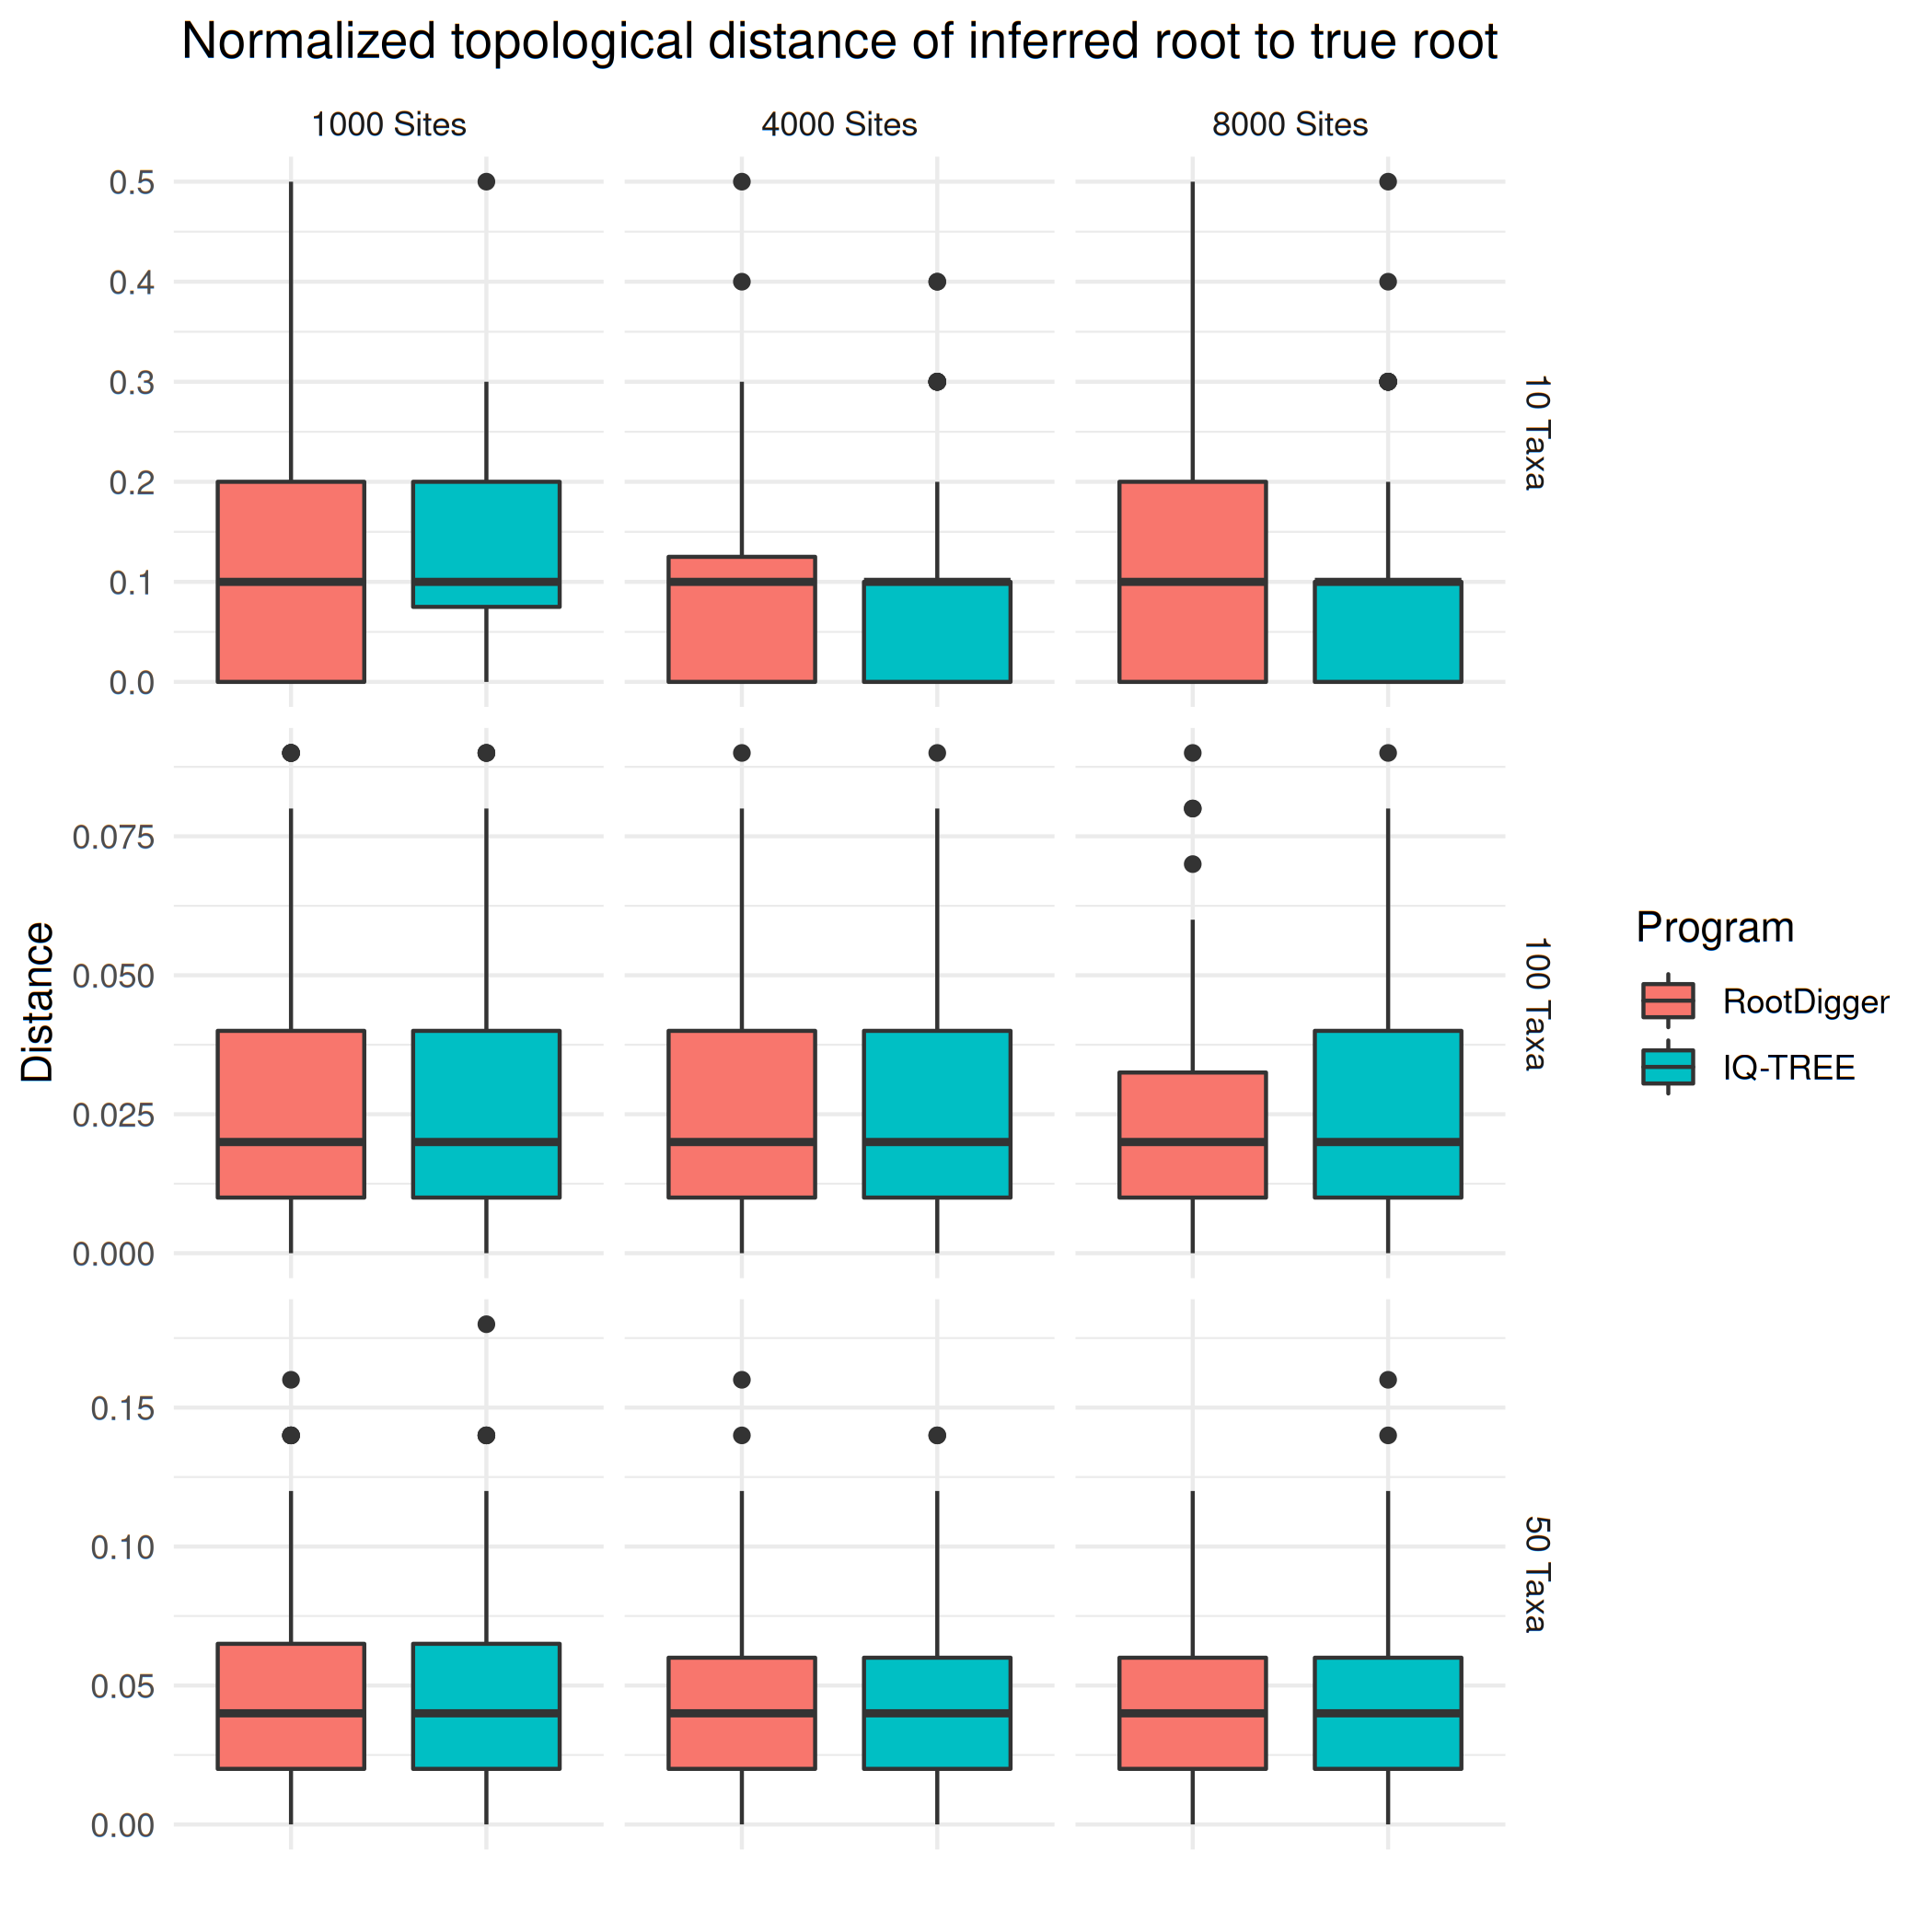
\includegraphics[width=.9\linewidth]{./figs/sim_results/melted_norm_dist_box.png}
%    \caption{Box plots of normalized topological error.
%    \label{fig:norm_error_boxplot}}
%\end{center}
%\end{figure}

\begin{figure}
  \begin{center}
    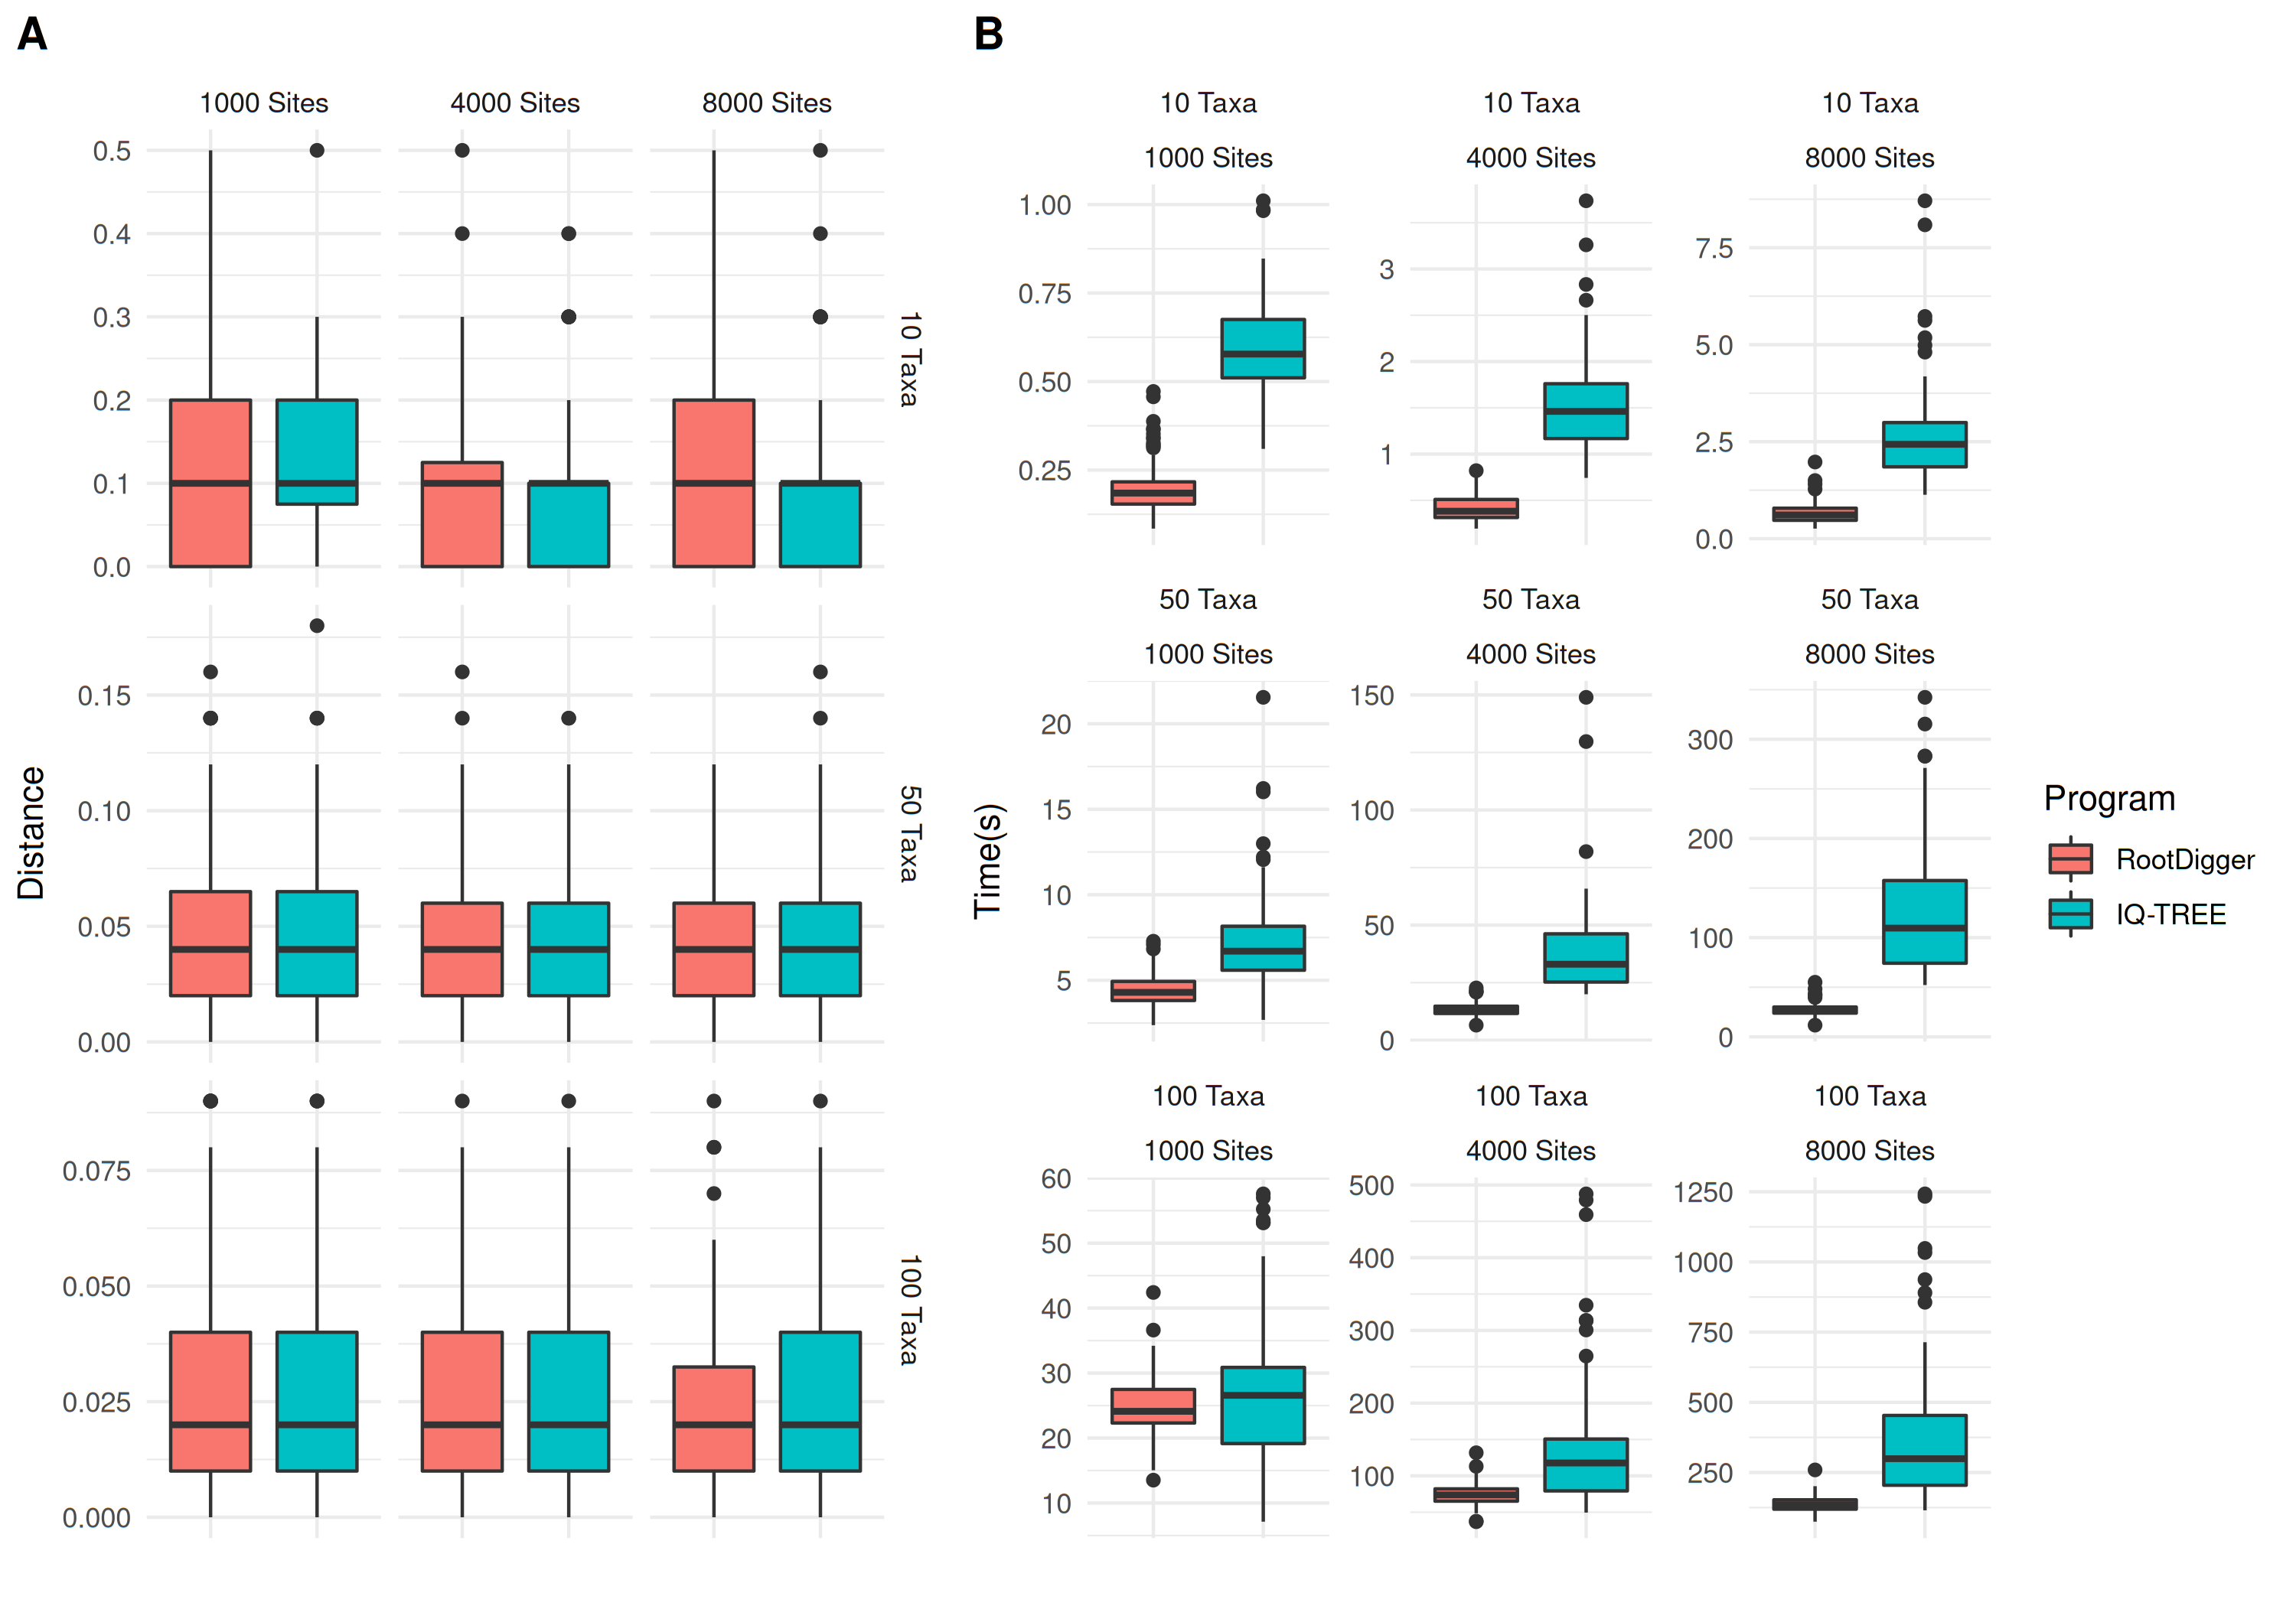
\includegraphics[width=\linewidth]{./figs/time_distance_boxplot.png}
    \caption{Comparison of \RootDiggertt{} and IQ-TREE on result error (A) and
      execution time (B). The distance in (A) is the topological distance from
      the placed root to the true root normalized by the number of taxa on the
      tree.
    \label{fig:timing-box-plot}}
\end{center}
\end{figure}

%\begin{figure}
%  \begin{center}
%    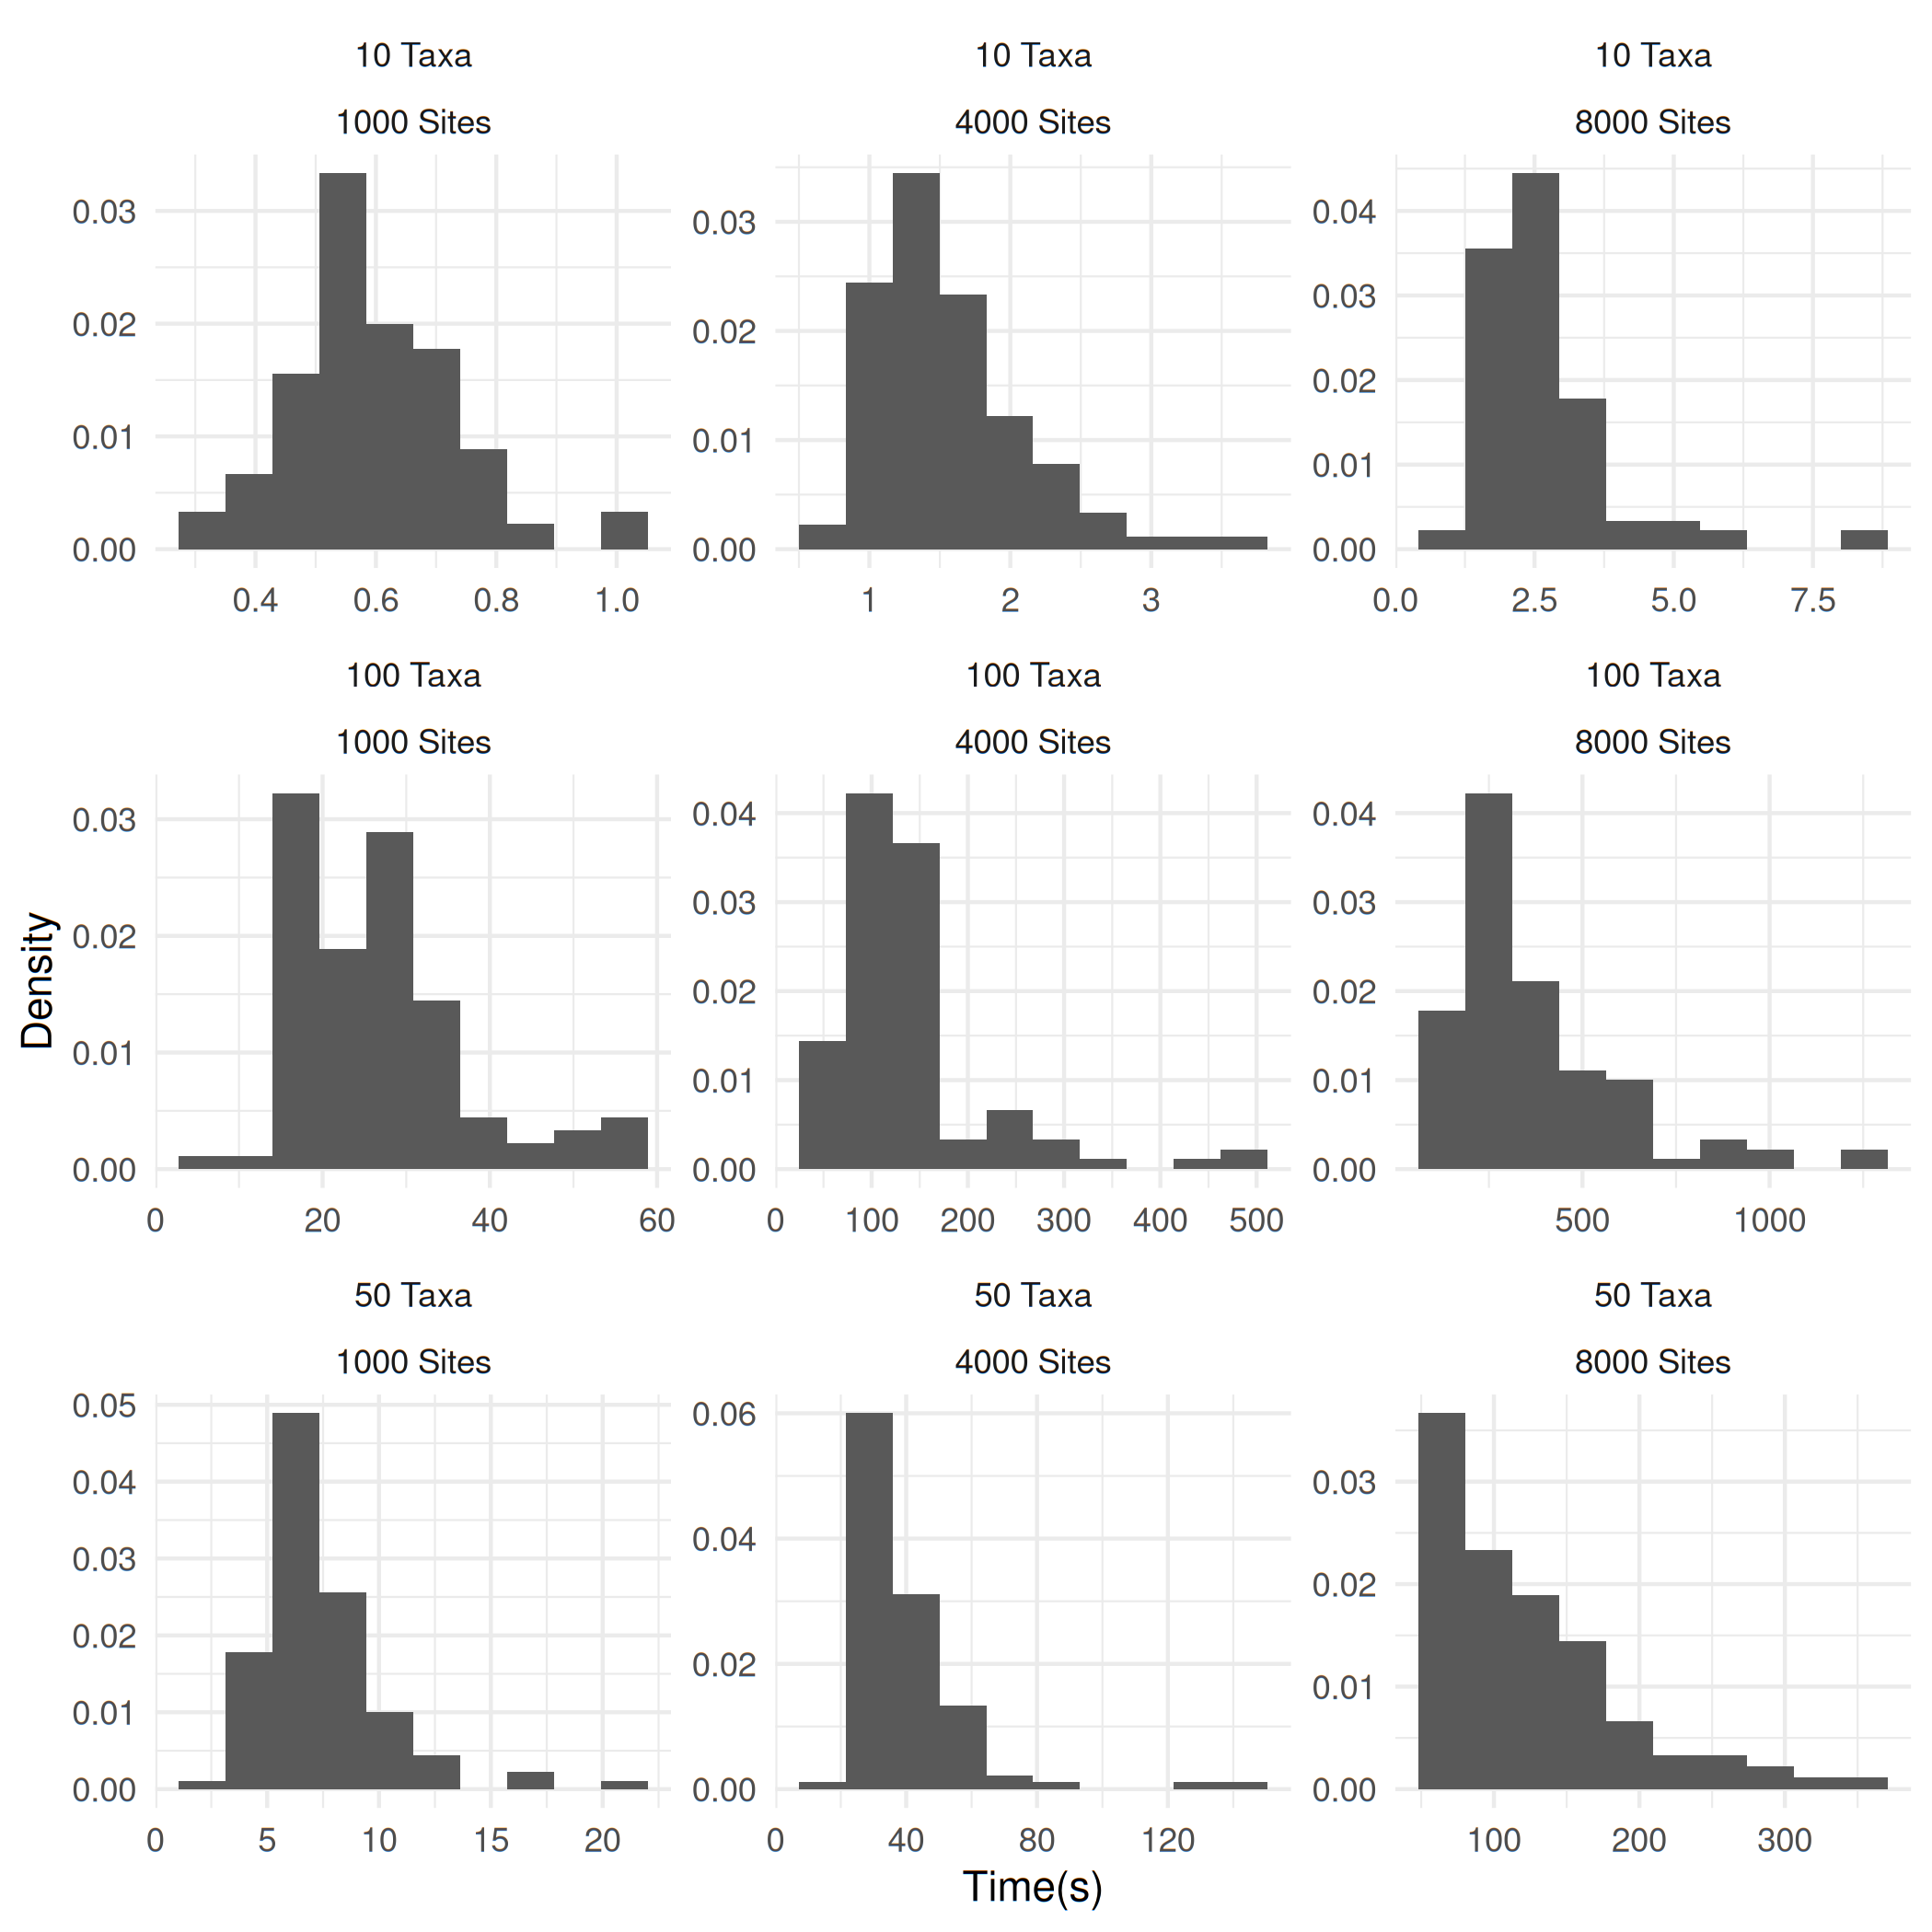
\includegraphics[width=.9\linewidth]{./figs/timing_plots/iq_time_hist.png}
%  \caption{Histogram of IQ-TREE times
%  \label{fig:iq_time_results}}
%\end{center}
%\end{figure}

%\begin{figure}
%  \begin{center}
%    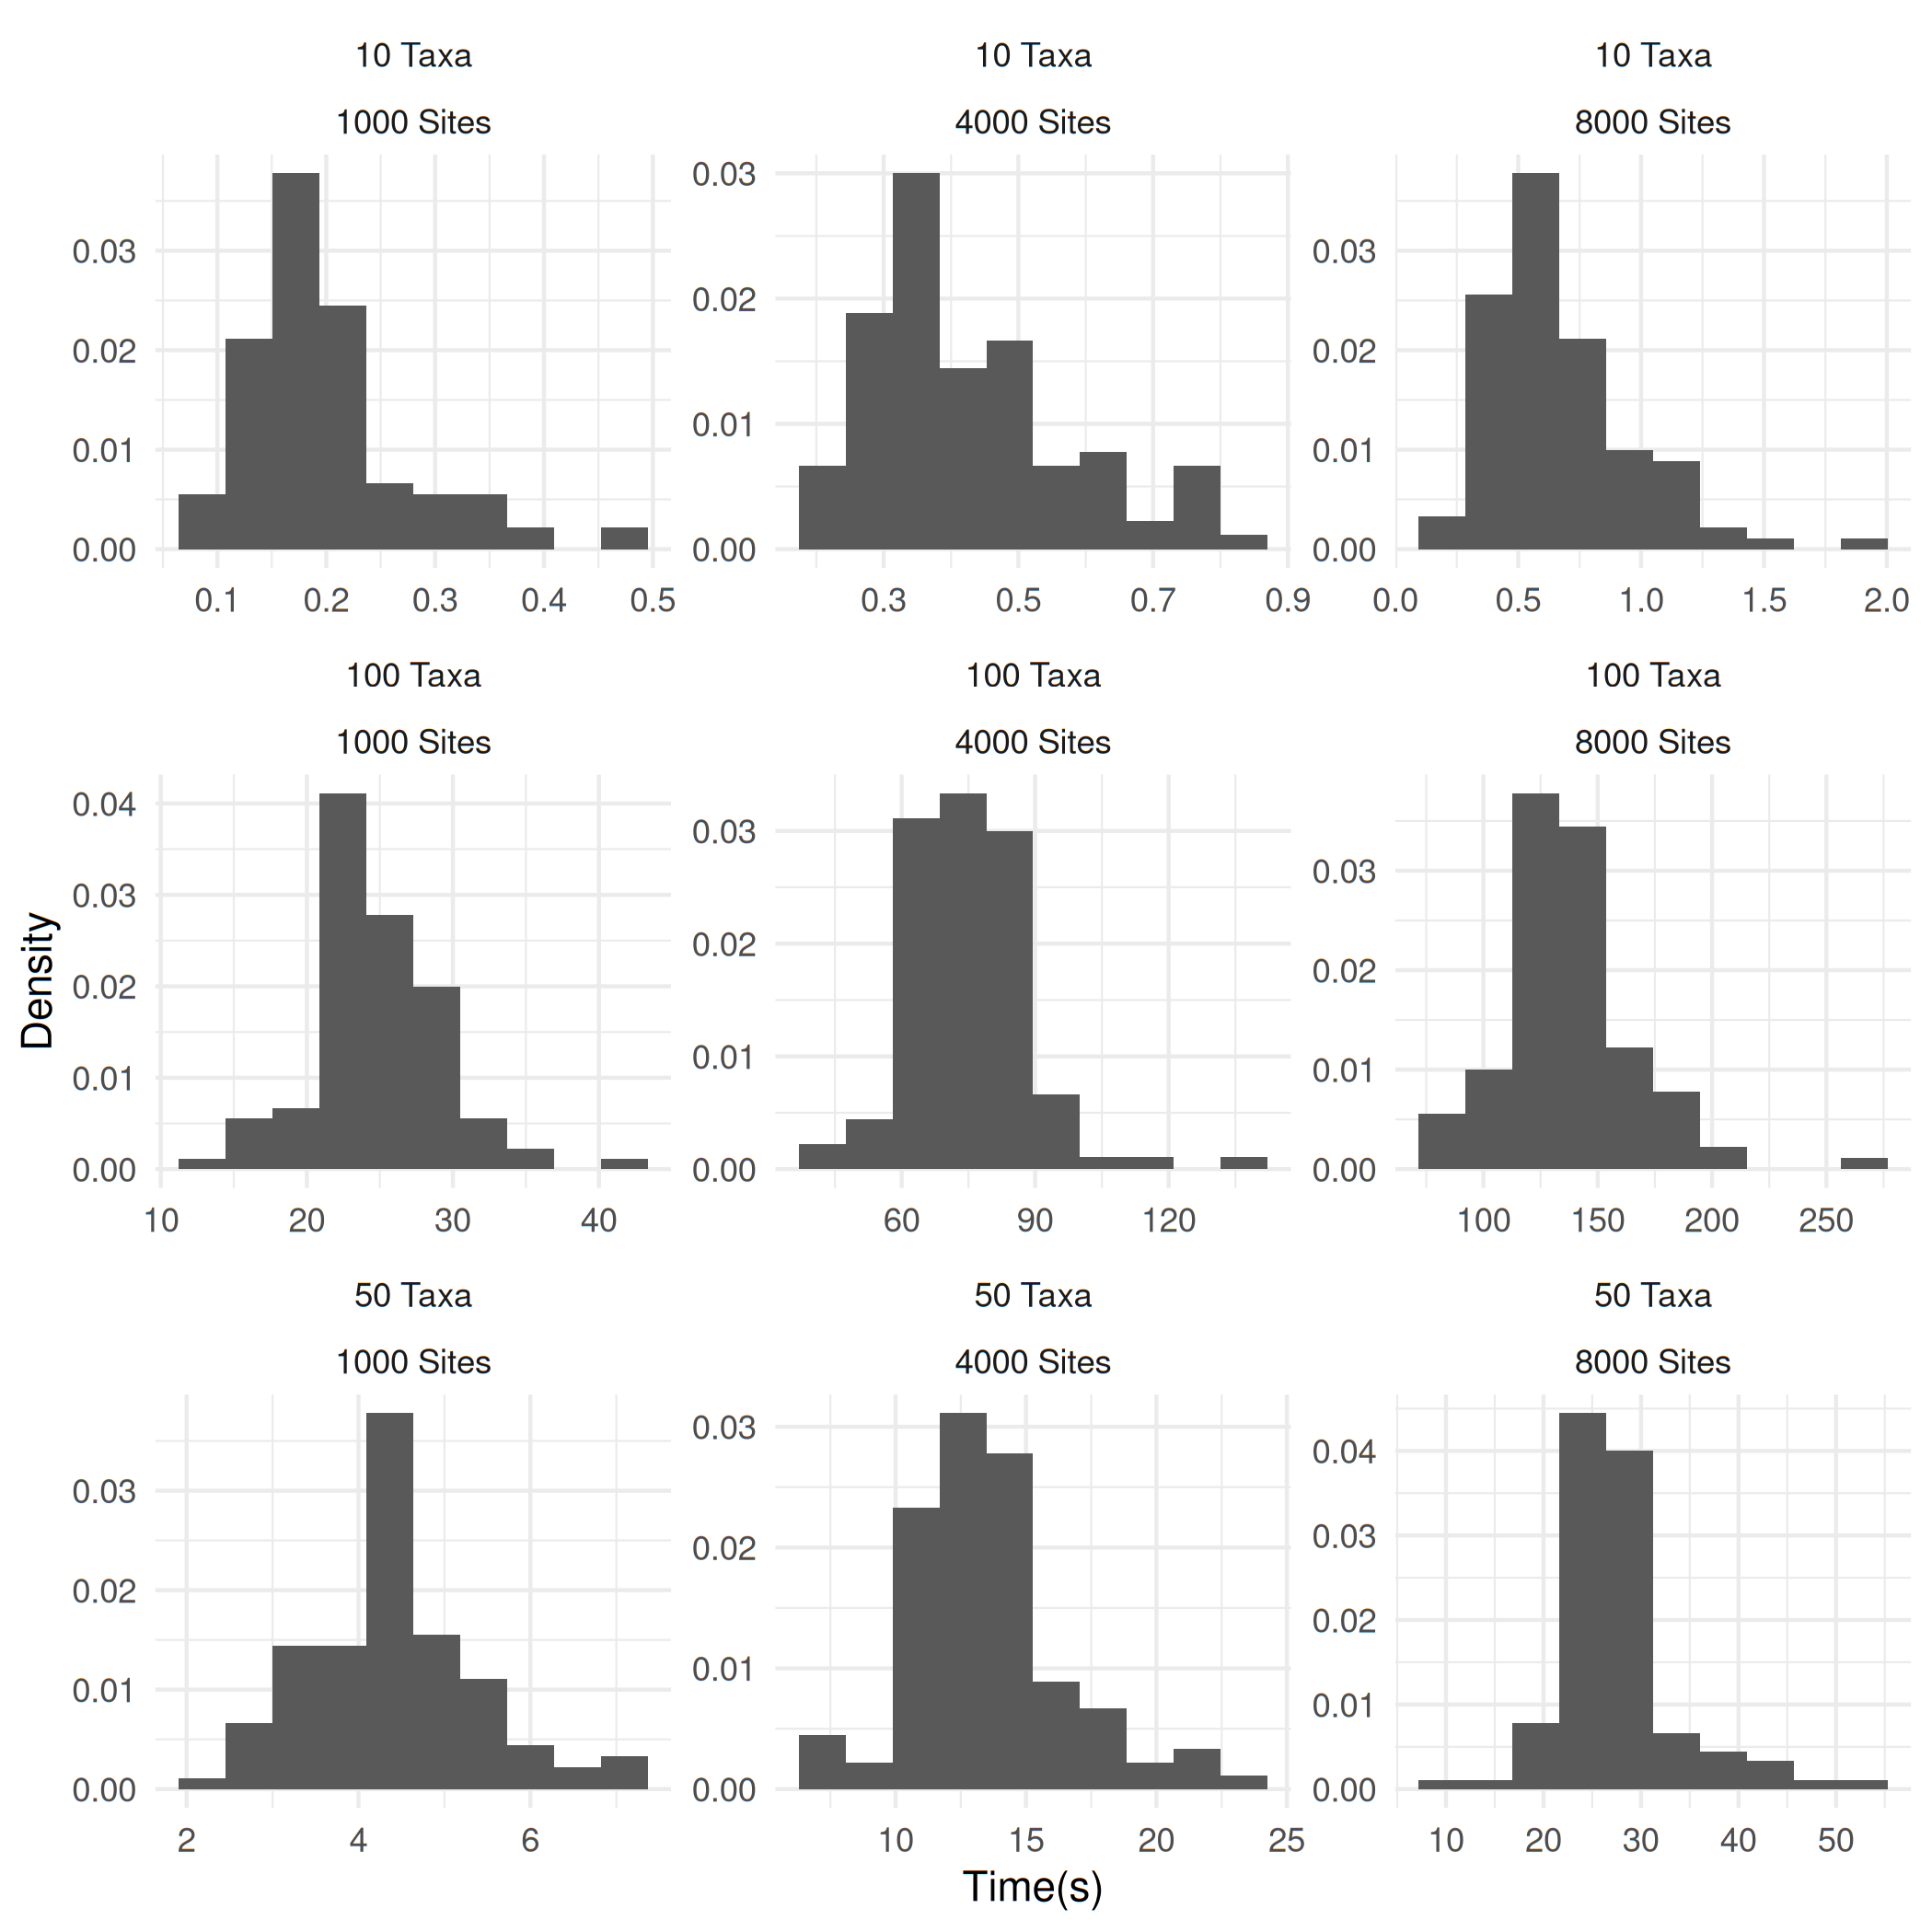
\includegraphics[width=.9\linewidth]{./figs/timing_plots/rd_time_hist.png}
%    \caption{Histogram of \RootDiggertt{} times
%    \label{fig:rd_time_results}}
%\end{center}
%\end{figure}

%\begin{figure}
%  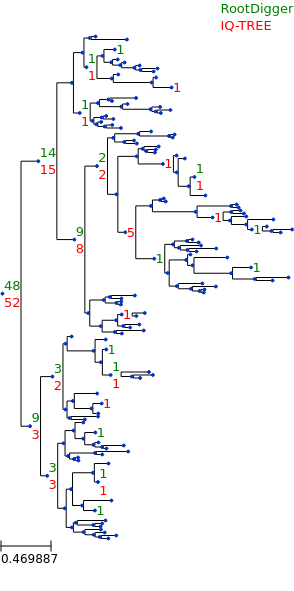
\includegraphics{figs/sim_results/100_1000.png}
%  \caption{Simulation results for 100 taxa and 1000
%  sites. \label{fig:sim-results-100t-1000s}}
%\end{figure}
%
%\begin{figure}
%  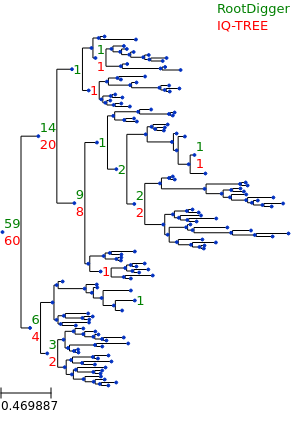
\includegraphics{figs/sim_results/100_8000.png}
%  \caption{Simulation results for 100 taxa and 8000
%  sites. \label{fig:sim-results-100t-8000s}}
%\end{figure}
%
%\begin{figure}
%  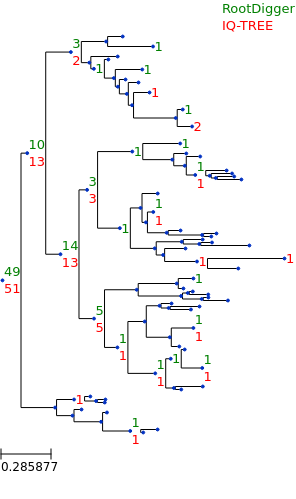
\includegraphics{figs/sim_results/50_1000.png}
%  \caption{Simulation results for 50 taxa and 1000
%  sites. \label{fig:sim-results-50t-1000s}}
%\end{figure}
%
%\begin{figure}
%  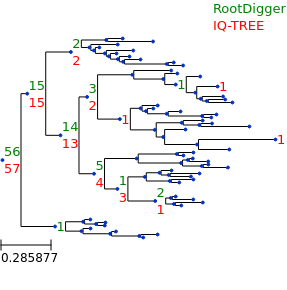
\includegraphics{figs/sim_results/50_8000.png}
%  \caption{Simulation results for 100 taxa and 8000
%  sites. \label{fig:sim-results-50t-8000s}}
%\end{figure}

\subsection{Empirical Data}

In addition to simulated data, we conducted tests with empirical data. The
datasets used are described in table~\ref{table:datasets}.  The empirical
datasets were chosen to have an existing, strongly supported outgroup.  For each
of the empirical datasets, we ran \RootDiggertt{} in exhaustive mode to obtain
likelihood weight ratios (LWR) for each branch.  Annotations are suppressed for
branches with a small LWR (less than $0.0001$).  The trees with annotated LWR
are shown in figures \ref{fig:spiders-missing-species-no-outgroup} -
\ref{fig:angio-cds12-outgroup}.  We ran the experiments on the datasets with the
outgroup included, as well as with the outgroup removed.

There was some preprocessing performed. In order to be sure branch lengths in
all datasets were specified in substitutions per site, the branch lengths were
re-optimized using RAxML-NG \cite{kozlov_raxml-ng:_2019} version
\texttt{0.9.0git}. The original model was used when it was
known\BenComment{which datasets}, otherwise the
branch lengths were optimized using GTR+G.

\begin{table}[H]
  \begin{center}
    \begin{tabular} { l c c c}
   Dataset & \#Taxa & \#Sites & Source \\
   \hline
   AngiospermsCDS12 & 35 & 864029 & \cite{ran_phylogenomics_2018}\\
   AngiospermsCDS & 35 & 1296043 & \cite{ran_phylogenomics_2018}\\
   Grasses & 245 & 4973 & \cite{christin_molecular_2014}\\
   Ficus & 200 & 5552 & \cite{cruaud_extreme_2012}\\
   SpidersMissingSpecies & 33 & 1097842 & \cite{leduc-robert_phylogeny_2018}\\
   SpidersMitocondrial & 34 & 12479 & \cite {leduc-robert_phylogeny_2018}\\
\end{tabular}
\caption{Table of emperical datasets used for validation}

    \label{table:datasets}
  \end{center}
\end{table}

%\begin{table}
%  \begin{center}
%    \begin{tabular} { l || c c  || c c  || c c || }
   Dataset & \multicolumn{2}{c ||}{Distance} & \multicolumn{2}{c ||}{Path Distance} &
   \multicolumn{2}{c ||}{Time} \\
           & RD & IQ & RD & IQ & RD & IQ \\
   \hline
   AngiospermsCDS12       & &  & & & &\\
   AngiospermsCDS         & &  & & & &\\
   Grasses                & &  & & & &\\
   Ficus                  & &  & & & &\\
   SpidersMissingSpecies  & &  & & & &\\
   SpidersMitocondrial    & &  & & & &\\
\end{tabular}
\caption{Results for empirical datasets. Distance is the distance from the
estimated root placement to the true root placement, taking into account branch
lengths. Path Distance is the topological distance from the estimated root
placement to the true root placement. RD Time and IQ time are the run times}

%    \label{table:emperical_results}
%  \end{center}
%\end{table}

%\begin{figure}
%  \begin{center}
%    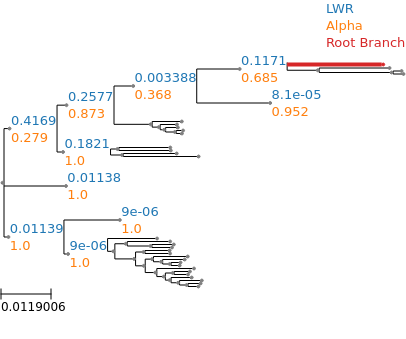
\includegraphics[width=.75\linewidth]{
%    ./figs/spiders/missing_species_no_outgroup.png}
%    \caption{SpidersMissingSpecies dataset analyzed without an outgroup.}
%    \label{fig:spiders-missing-species-no-outgroup}
%  \end{center}
%\end{figure}

%\begin{figure}
%  \begin{center}
%    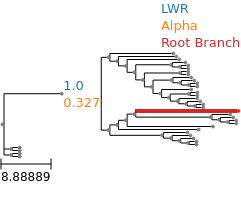
\includegraphics[width=.75\linewidth]{
%    ./figs/spiders/missing_species_with_outgroup.png}
%    \caption{SpidersMissingSpecies dataset analyzed with an outgroup.}
%    \label{fig:spiders-missing-species-outgroup}
%  \end{center}
%\end{figure}

%\begin{figure}
%  \begin{center}
%    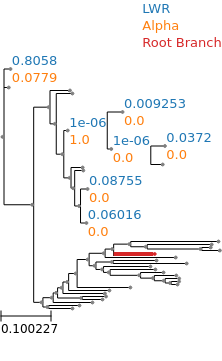
\includegraphics[width=.75\linewidth]{./figs/spiders/mito_no_outgroup.png}
%    \caption{SpidersMitocondrial dataset analyzed without an outgroup.}
%    \label{fig:spiders-mito-no-outgroup}
%  \end{center}
%\end{figure}

%\begin{figure}
%  \begin{center}
%    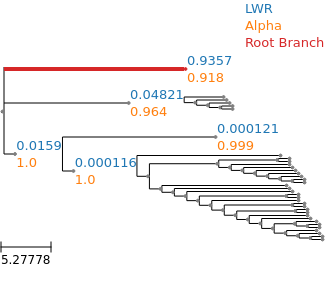
\includegraphics[width=.75\linewidth]{./figs/spiders/mito_with_outgroup.png}
%    \caption{SpidersMitocondrial dataset analyzed with an outgroup.}
%    \label{fig:spiders-mito-outgroup}
%  \end{center}
%\end{figure}

%\begin{figure}[H]
%  \begin{center}
%    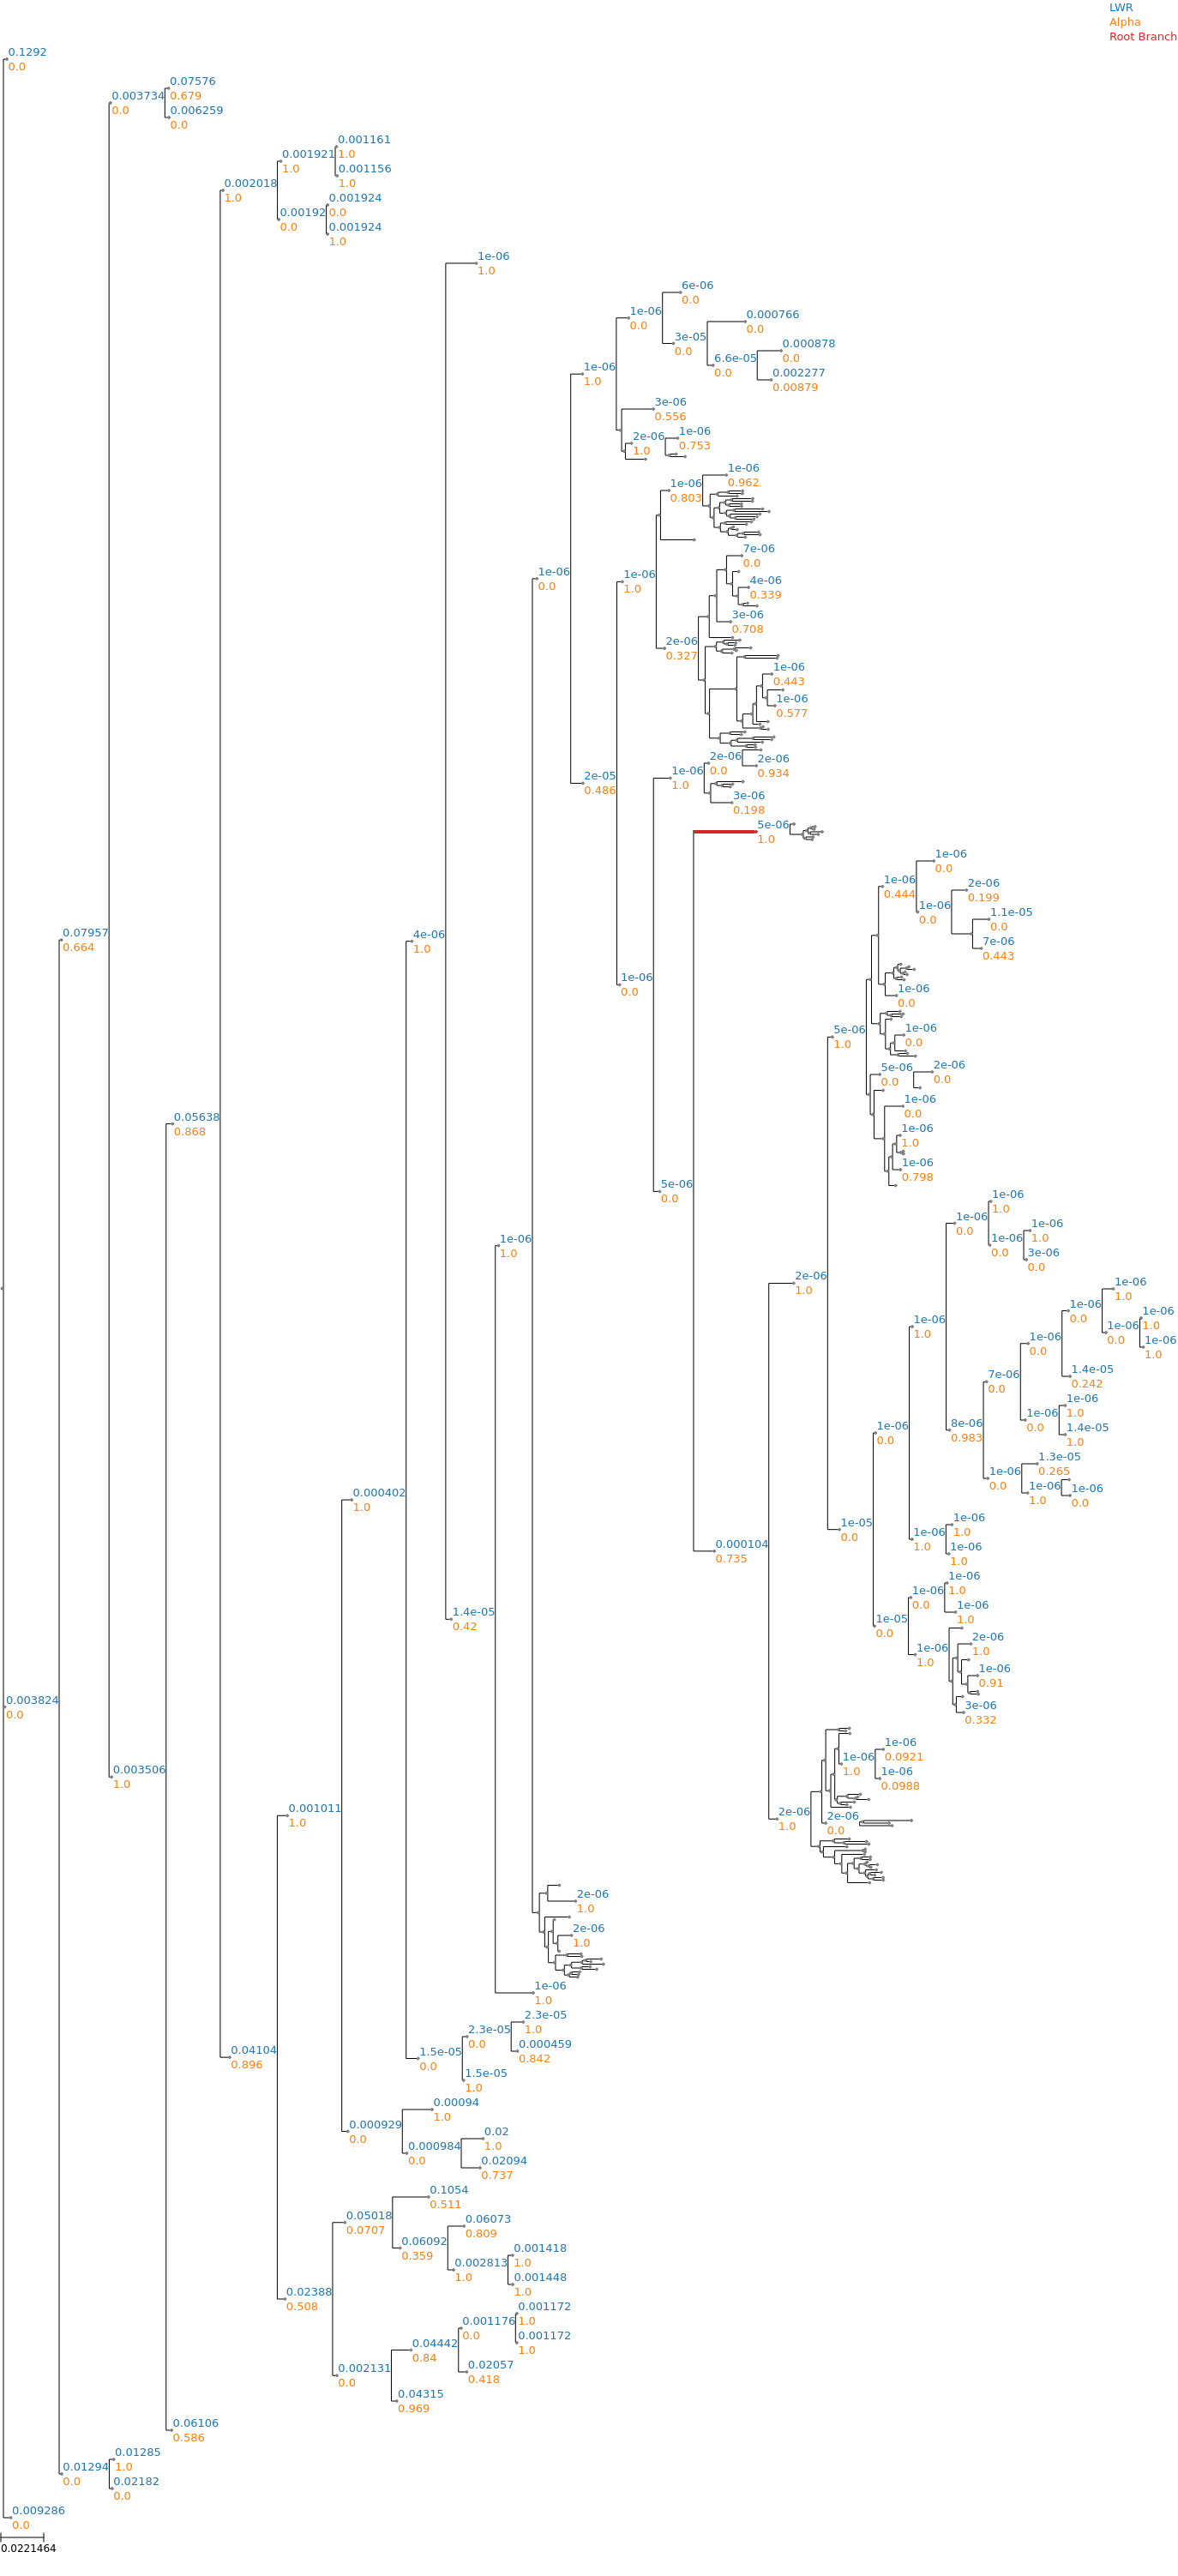
\includegraphics[width=.75\linewidth]{figs/ficus/ficus_no_outgroup.png}
%    \caption{Ficus dataset analyzed without an outgroup.}
%    \label{fig:ficus-no-outgroup}
%  \end{center}
%\end{figure}
%
%\begin{figure}[H]
%  \begin{center}
%    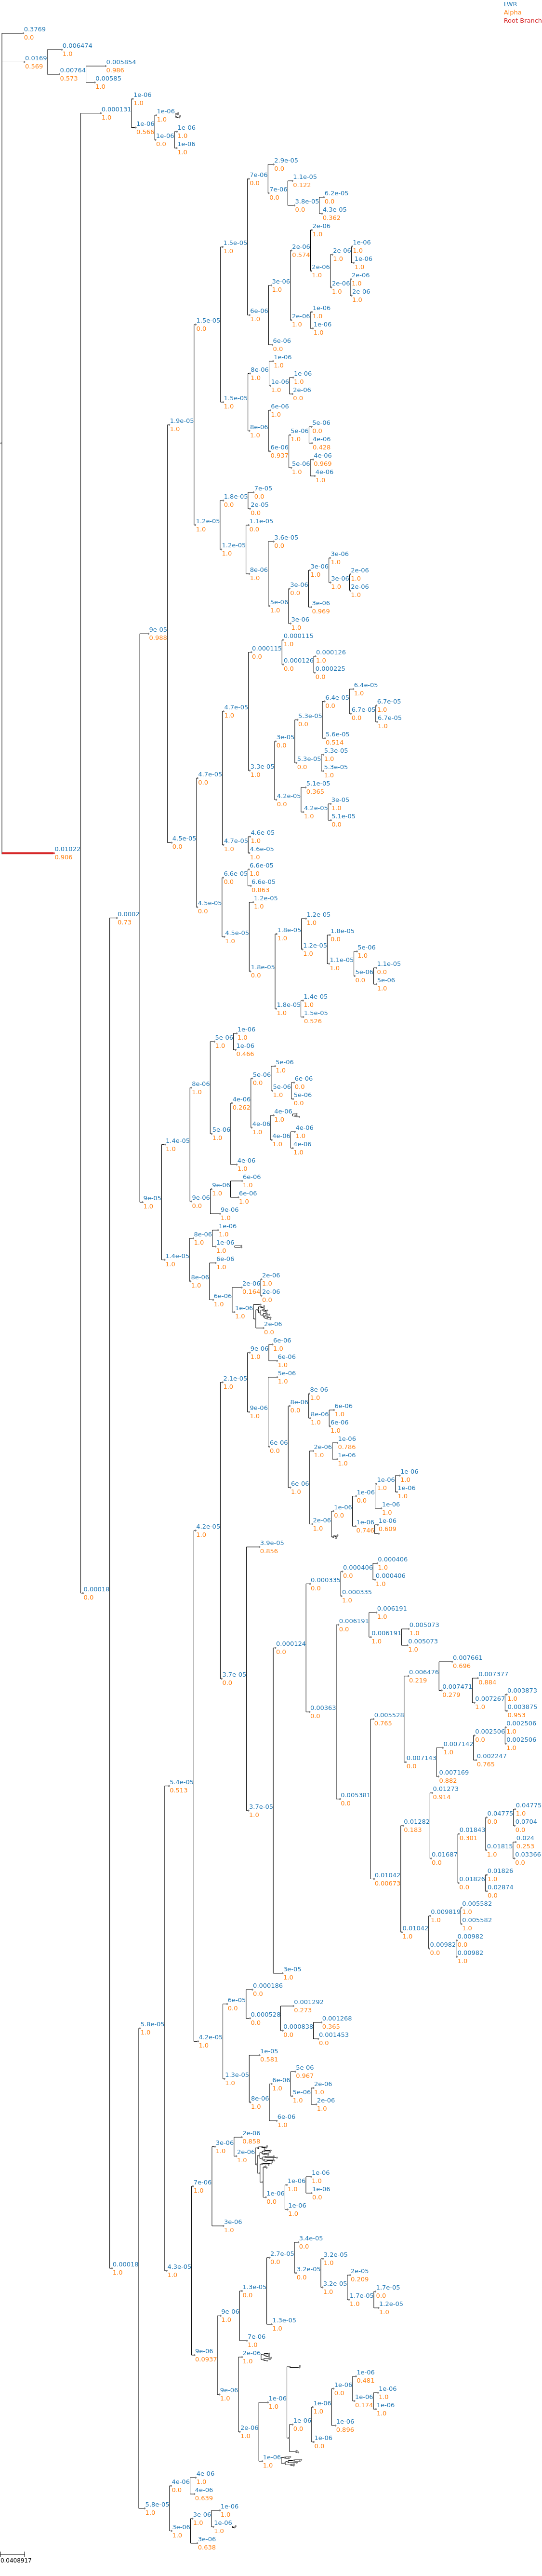
\includegraphics[width=.75\linewidth]{figs/ficus/ficus_with_outgroup.png}
%    \caption{Ficus dataset analyzed with an outgroup.}
%    \label{fig:ficus-outgroup}
%  \end{center}
%\end{figure}

%\begin{figure}
%  \begin{center}
%    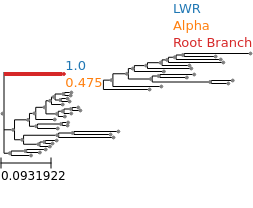
\includegraphics[width=.5\linewidth]{figs/angio/cds12_no_outgroup.png}
%    \caption{AngiospermsCDS12 dataset analyzed without an outgroup.}
%    \label{fig:angio-cds12-no-outgroup}
%  \end{center}
%\end{figure}
%
%\begin{figure}
%  \begin{center}
%    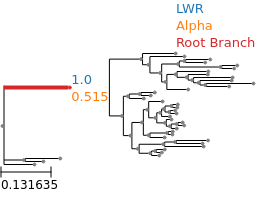
\includegraphics[width=.5\linewidth]{./figs/angio/cds12_with_outgroup.png}
%    \caption{AngiospermsCDS12 dataset analyzed with an outgroup.}
%    \label{fig:angio-cds12-outgroup}
%  \end{center}
%\end{figure}
%
%\begin{figure}
%  \begin{center}
%    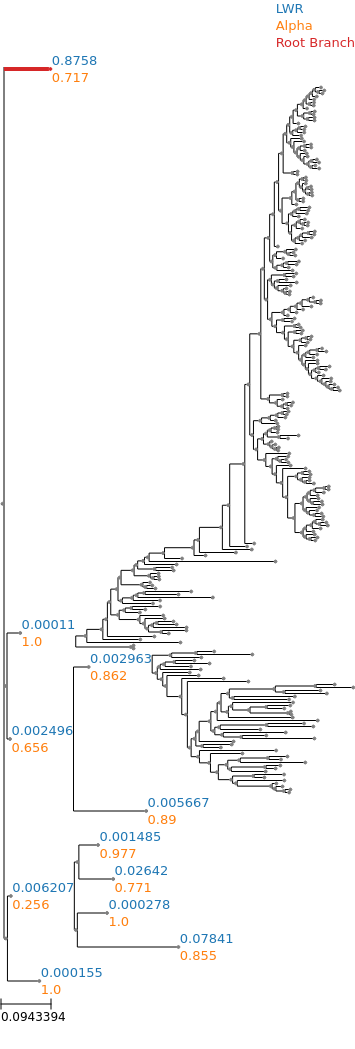
\includegraphics[width=.5\linewidth]{./figs/grasses/plastid245_no_outgroup.png}
%    \caption{Grasses dataset analyzed without an outgroup.}
%    \label{fig:grasses}
%  \end{center}
%\end{figure}

%\begin{figure}[H]
%  \begin{center}
%    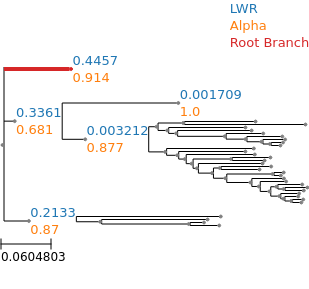
\includegraphics[width=.4\linewidth]{figs/spiders/1rate.png}
%    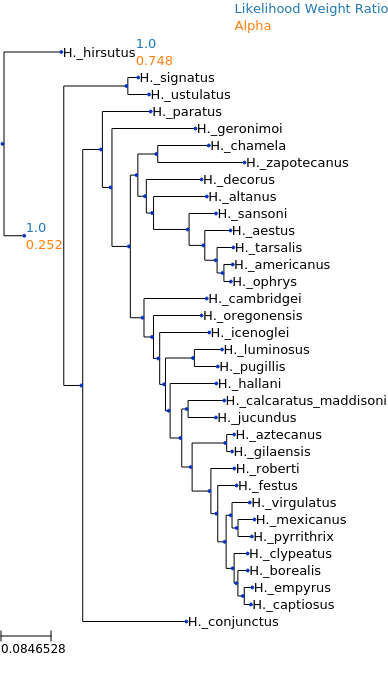
\includegraphics[width=.4\linewidth]{figs/spiders/2rate.png}
%    \caption{SpidersMitocondrial dataset analyzed with varying rate categories.
%    Left is with 1 rate category, and right is with 2.}
%    \label{fig:spiders-rate-compare}
%  \end{center}
%\end{figure}

\subsection{Effect of early stopping on result}

Finally, we investigated the effect of the early stopping criterion on the final
LWR results. To do this, we ran \RootDiggertt{} in exhaustive mode on all
empirical datasets with early stopping enabled and disabled, resulting in paired
runs which could be compared. For most runs, the results with and without early
stopping showed no meaningful (difference in LWR less than $0.000001$)
difference. The dataset that showed the largest difference in LWR is shown in
figure \ref{fig:es_mito}. In exchange, the runtime of this dataset with early
stop enabled is roughly 1.7 times faster.


%\begin{figure}[H]
%  \begin{center}
%    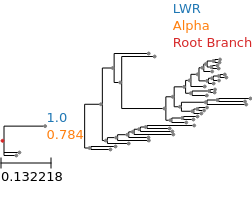
\includegraphics[width=.4\linewidth]{figs/early_stop_tests/es_test_cds12_no_outgroup.png}
%    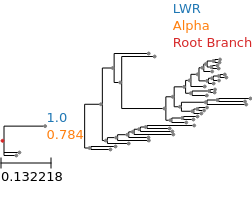
\includegraphics[width=.4\linewidth]{figs/early_stop_tests/es_test_cds12_no_outgroup_noes.png}
%    \caption{Effect of early stopping on results. Left is with early stopping,
%    Left is without. Dataset is AngiospermsCDS12}
%    \label{fig:es_angio}
%  \end{center}
%\end{figure}
\begin{figure}[H]
  \begin{center}
    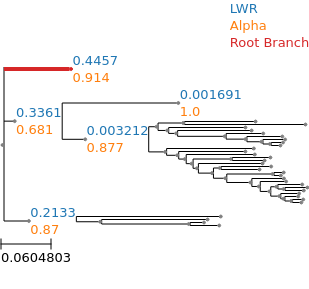
\includegraphics[width=.4\linewidth]{figs/early_stop_tests/es_test_mito_no_outgroup.png}
    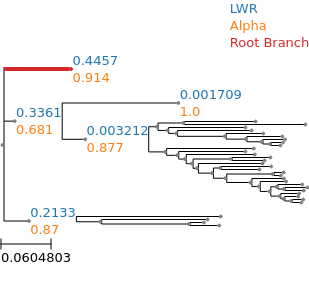
\includegraphics[width=.4\linewidth]{figs/early_stop_tests/es_test_mito_no_outgroup_noes.png}
    \caption{Effect of early stopping on results. Left is with early stopping,
    Right is without. Dataset is SpidersMitocondrial and has the largest
  observed difference.}
    \label{fig:es_mito}
  \end{center}
\end{figure}

\section{Discussion}

%TOPICS:
% - Adaptive number of roots for search mode.

\RootDiggertt{} is substantially faster than IQ-TREE, as is shown when comparing
figure~\ref{fig:timing-box-plot}. Furthermore, the accuracy of root placement of
\RootDiggertt{} is nearly the same as IQ-TREE, as seen in
figure~\ref{fig:timing-box-plot}.  Early stopping proved to be an effective
technique to reduce execution times at an extremely marginal cost in accuracy.
The largest observed difference on empirical datasets between using early stop
mode and is negligent, as it can be seen in figure~\ref{fig:es_mito}. 

In Huelsenbeck \cite{huelsenbeck_inferring_2002}, it was shown that the prior
probability of a root placement on a sample tree did not have a strong signal
when using a non-reversible model of character substitution.  While performing
our verification of \RootDiggertt{} using empirical data, we found that this was
often not the case. For example on the AngiospermsCDS12 dataset (see figure
\ref{fig:angio-cds12-no-outgroup}), we found a clear signal for the root
placement, both with and without the outgroup. Even in cases when the signal was
not as strong, for example SpidersMitocondrial (see figure
\ref{fig:spiders-mito-no-outgroup}), there is a much stronger signal for root
placement than Huelsenbeck would suggest we would get with this kind of analysis
(which is to say, analysis using a non-reversible model). The one exception to
this is the ficus dataset, which showed at least marginal support for the root
on nearly all branches of the tree. We suspect that this is due to Huelsenbeck
performing the analysis on a 4 taxon tree with the distantly related taxa frog,
bird, mouse, and human. By only using 4 distantly related taxa, the rate matrix
is less constrained by the data present, which leads to over fitting the rate
matrix.  It is our opinion that the methods presented here will usually produce
a clear signal for the rooting of a tree, and that the analysis in Huelsenbeck
was incomplete.

\section{Conclusion}

We have shown that some datasets are particularly well suited to this form of
analysis, and that \RootDiggertt{} can be a simple alternative to similar forms
of root inference, such as molecular clock analysis or the use of an outgroup.

\section{Future Work}

Going forward with \RootDiggertt{}, there are several developments that would be
useful. One of these is support for more models. Currently we support only the
most complicated model UNREST, but in the future it might be useful to support
less complicated models, such as the Lie group models described in
Woodhams~\cite{woodhams_new_2015}.  In particular, models with fewer parameters
are generally regarded as being less prone to over fitting, which would lead to
a better assessment of the true root location.

In addition to more models, other data types could be supported, particular
amino acid (AA) data. In this work, we decided not to use AA data as it would
bring the number of free parameters from 12 for DNA data to $380$ for AA. We
suspect that this number of parameters is far too prone to over fitting to be
useful, but that was never truly investigated.

Finally, there are a few parameters that are not part of the model that could be
heuristically set. These parameters include the number of initial candidate
roots in the search mode, the number of roots to fully optimize during each step
of the search mode. In this work these parameters were selected to be well
performing on simulations, but better results could possibly be obtained from an
adaptive strategy.

\bibliographystyle{acm}
\bibliography{main}

\end{document}
